\documentclass[ignorenonframetext,aspectratio=43]{beamer}
\setbeamertemplate{caption}[numbered]
\setbeamertemplate{caption label separator}{: }
\setbeamercolor{caption name}{fg=normal text.fg}
\beamertemplatenavigationsymbolsempty
\usepackage{lmodern}
\usepackage{amssymb,amsmath}
\usepackage{ifxetex,ifluatex}
\usepackage{fixltx2e} % provides \textsubscript
\ifnum 0\ifxetex 1\fi\ifluatex 1\fi=0 % if pdftex
  \usepackage[T1]{fontenc}
  \usepackage[utf8]{inputenc}
\else % if luatex or xelatex
  \ifxetex
    \usepackage{mathspec}
  \else
    \usepackage{fontspec}
  \fi
  \defaultfontfeatures{Ligatures=TeX,Scale=MatchLowercase}
\fi
% use upquote if available, for straight quotes in verbatim environments
\IfFileExists{upquote.sty}{\usepackage{upquote}}{}
% use microtype if available
\IfFileExists{microtype.sty}{%
\usepackage{microtype}
\UseMicrotypeSet[protrusion]{basicmath} % disable protrusion for tt fonts
}{}
\newif\ifbibliography
\usepackage{color}

\usepackage{graphicx,grffile}
\makeatletter
\def\maxwidth{\ifdim\Gin@nat@width>\linewidth\linewidth\else\Gin@nat@width\fi}
\def\maxheight{\ifdim\Gin@nat@height>\textheight0.8\textheight\else\Gin@nat@height\fi}
\makeatother

% Prevent slide breaks in the middle of a paragraph:
\widowpenalties 1 10000
\raggedbottom

\AtBeginPart{
  \let\insertpartnumber\relax
  \let\partname\relax
  \frame{\partpage}
}
\AtBeginSection{
  \ifbibliography
  \else
    \let\insertsectionnumber\relax
    \let\sectionname\relax
    \frame{\sectionpage}
  \fi
}
\AtBeginSubsection{
  \let\insertsubsectionnumber\relax
  \let\subsectionname\relax
  \frame{\subsectionpage}
}

\setlength{\parindent}{0pt}
\setlength{\parskip}{6pt plus 2pt minus 1pt}
\setlength{\emergencystretch}{3em}  % prevent overfull lines
\providecommand{\tightlist}{%
  \setlength{\itemsep}{0pt}\setlength{\parskip}{0pt}}
\setcounter{secnumdepth}{0}
\DeclareUnicodeCharacter{00A0}{~}
\DeclareUnicodeCharacter{03B4}{$\delta$}
\DeclareUnicodeCharacter{03B5}{$\varepsilon$}
\DeclareUnicodeCharacter{03C9}{$\omega$}
\DeclareUnicodeCharacter{2124}{\mathbb{Z}}
\DeclareUnicodeCharacter{2193}{$\downarrow$}
\DeclareUnicodeCharacter{2208}{$\in$}
\DeclareUnicodeCharacter{2209}{$\notin$}
\DeclareUnicodeCharacter{220B}{$\ni$}
\DeclareUnicodeCharacter{2227}{$\wedge$}
\DeclareUnicodeCharacter{2228}{$\vee$}
\DeclareUnicodeCharacter{2234}{$\therefore$}
\DeclareUnicodeCharacter{2264}{$\leq$}
\DeclareUnicodeCharacter{2265}{$\geq$}
\DeclareUnicodeCharacter{2605}{$\star$}
\DeclareUnicodeCharacter{1D53D}{\mathbb{F}}

% Scale images if necessary, so that they will not overflow the page
% margins by default, and it is still possible to overwrite the defaults
% using explicit options in \includegraphics[width, height, ...]{}
%\setkeys{Gin}{width=\maxwidth,height=\maxheight,keepaspectratio}
\newcommand{\includegraphicsscaled}[1]{
    \includegraphics[width=\maxwidth,height=\maxheight,keepaspectratio]{#1}
}

\usefonttheme[onlymath]{serif}
\hypersetup{breaklinks=true,colorlinks,linkcolor=,urlcolor=purple}
\setbeamertemplate{navigation symbols}{}
\setbeamercolor{footnote mark}{fg=gray}
\setbeamerfont{footnote}{size=\tiny}
\usepackage[normalem]{ulem}
\usepackage{listings}
\lstset{
    basicstyle=\ttfamily\large,
    keywordstyle=\color{blue}\bfseries,
    commentstyle=\color[rgb]{0,0.5,0}\bfseries\em
}

\newcommand\greyuline{\bgroup\markoverwith
    {\textcolor{lightgray}{\rule[-0.5ex]{2pt}{0.4pt}}}\ULon}

\title{\bf No way, JOSE!}
\subtitle{\bf Lessons for authors and implementers of open standards}
\author{\bf Fraser Tweedale\\
    \texttt{@hackuador}}
\date{\bf July 3, 2018}

%\setbeamertemplate{background}{
%  \ifnum\thepage<2%
%   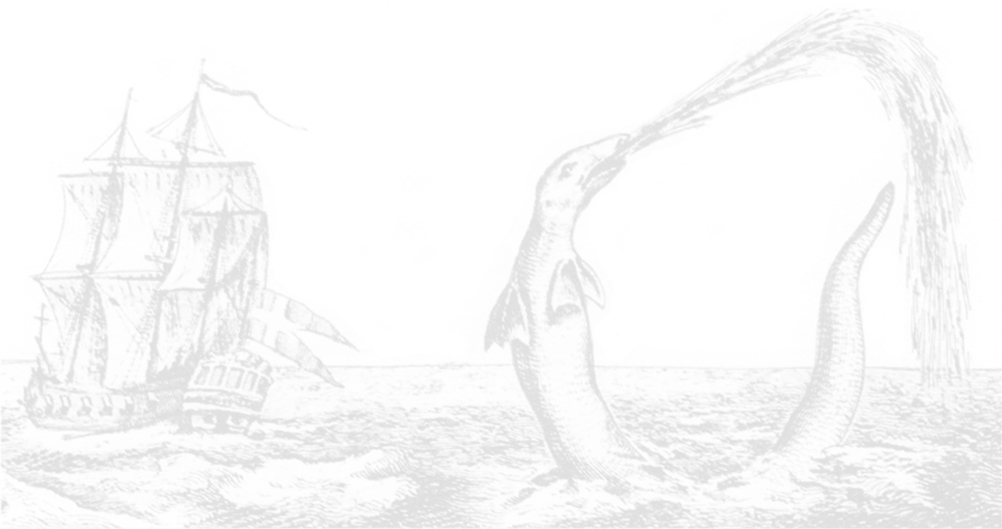
\includegraphics[height=\paperheight,width=\paperwidth]{Hans_Egede_sea_serpent_1734-light.jpg}
%  \fi
%}

\begin{document}

\begin{frame}
\titlepage
\end{frame}

\section{Introduction}\label{introduction}

\begin{frame}
\huge
A journey\ldots
\end{frame}

\begin{frame}{JOSE}
\begin{itemize}
\tightlist
\item \underline{\bf J}SON \underline{\bf O}bject
      \underline{\bf S}igning and \underline{\bf E}ncryption
\item IETF WG formed 2011, RFCs 2015
\item used in OpenID Connect, ACME
\end{itemize}
\end{frame}

\begin{frame}{JOSE \& me}
\begin{itemize}
\tightlist
\item I wrote a JOSE library for Haskell
\item I participated in IETF discussions
\item JOSE has lots of problems (sorry\ldots)
\end{itemize}
\end{frame}

\begin{frame}
\huge What is a standard?
\end{frame}



\section{Do you need a new standard?}

\begin{frame}{JOSE---rationale}
\begin{quotation}
\Large
  With the increased usage of JSON in protocols in the IETF and
  elsewhere, there is now a desire to offer security services, which use
  encryption, digital signatures, message authentication codes (MACs)
  algorithms, that carry their data in JSON format.\footnote[frame]{
    \url{https://tools.ietf.org/wg/jose/charters}}
\end{quotation}
% TODO highlight/emph for important parts of quotes

\end{frame}

\begin{frame}{JOSE---rationale}
% FIXME is this from RFC or Charter?
\begin{quotation}
\Large
  Many current applications thus have {\bf \em much more robust support} for
  processing objects in these text-based formats than ASN.1 objects;
  indeed, many {\bf \em lack the ability to process ASN.1} objects at all.  To
  {\bf \em simplify} the addition of object-based security features to these
  applications, the %IETF JSON Object Signing and Encryption (JOSE)
  working group has been chartered to develop a {\bf \em secure} object format
  based on JSON.\footnote[frame]{
    \url{https://tools.ietf.org/html/rfc7165}}
\end{quotation}
\end{frame}

\begin{frame}[plain]
\begin{center}
\includegraphicsscaled{standards.png}
\end{center}
\tiny CC BY-NC 2.5 \url{https://xkcd.com/927/}
\end{frame}

% fun fact: JOSE was originally "WOES": Web Object Encryption and Signing

\begin{frame}{JOSE---assumptions}
\begin{itemize}
\tightlist
\item ASN.1 libraries don't exist
\item It's better to define new standard than write a library
\item JSON is suitable for security/cryptographic objects
\item ASN.1 is bad
\end{itemize}
\end{frame}

\begin{frame}[fragile]{JOSE---irony}
\begin{verbatim}
4.7.  "x5c" (X.509 Certificate Chain) Parameter

   The "x5c" (X.509 certificate chain) parameter
   contains a chain of one or more PKIX certificates
   [RFC5280].  The certificate chain is represented
   as a JSON array of certificate value strings.
   Each string in the array is a base64-encoded
   (Section 4 of [RFC4648] -- not base64url-encoded)
   DER [ITU.X690.1994] PKIX certificate value.
\end{verbatim}
\end{frame}



\begin{frame}[plain]
\huge
Takeaway: write libraries, not standards
\end{frame}





\section{Is JSON the right choice?}

\begin{frame}[plain]
\huge
Falsehoods programmers believe about JSON\ldots
\end{frame}

\begin{frame}[plain]
\huge
JSON support is universal.
\end{frame}

\begin{frame}[plain]
\LARGE \centering
C \\
Rust \\
C++ \\
Scala \\
Haskell \\
\ldots
\end{frame}
% (with json support) python ruby js, Java EE, CLI (.NET)

\begin{frame}[plain]
\huge
JSON is human readable.
\end{frame}

\begin{frame}[fragile]
\begin{lstlisting}[language=]
{"signature":"M3oVLXrbeFRT9Ef9d3WzR-D7dGtI
eYoPBYmiCdtYqus","protected":"eyJhbGciOiJI
UzI1NiIsImtpZCI6ImthcmF0ZSJ9","payload":"e
yJzdWJqZWN0IjoiZnJhc2VAZnJhc2UuaWQuYXUiLCJ
pc3MiOiJocy1qb3NlIiwiYXVkIjpbImFsaWNlIiwiY
m9iIl19Cg"}
\end{lstlisting}
\end{frame}

\begin{frame}[plain]
\huge
JSON is unambiguously specified.
\end{frame}

\begin{frame}{JSON---ambiguities}
\begin{itemize}
\tightlist
\item invalid code points
\item data size limits
\end{itemize}
\end{frame}

\begin{frame}[plain]
\huge
JSON objects are maps.
\end{frame}

\begin{frame}{JSON---objects}
\begin{itemize}
\tightlist
\item \texttt{names within an object SHOULD be unique}---RFC 8259
\item Is a JSON object a map?
\item What {\em kind} of map?
\item How should duplicate keys be treated?
\end{itemize}
\end{frame}

\begin{frame}[plain]
\huge
JSON will be parsed the same way by different parsers.
\end{frame}

\begin{frame}[plain]
\begin{center}
\includegraphicsscaled{pruned_results.png}
\end{center}
\tiny \url{http://seriot.ch/parsing_json.php}
\end{frame}

\begin{frame}
\centering
\LARGE
CVE-2017-12635
\end{frame}
% https://justi.cz/security/2017/11/14/couchdb-rce-npm.html
% https://cve.mitre.org/cgi-bin/cvename.cgi?name=2017-12635
% https://www.exploit-db.com/exploits/44498/
% python exploit snippet
% cu_data_payload = '{"type": "user", "name": "'+user+'", "roles": ["_admin"], "roles": [], "password": "'+password+'"}'

\begin{frame}{JSON---other problems}
\begin{itemize}
\tightlist
\item ``number''
\item binary data
\item no canonical serialisation
\end{itemize}
\end{frame}

\begin{frame}[plain]
\begin{center}
\includegraphicsscaled{yo-dawg.jpg}
\end{center}
\end{frame}

\begin{frame}{JSON---alternatives}
\begin{itemize}
\tightlist
\item ASN.1
\item CBOR
\end{itemize}
\end{frame}

\begin{frame}[plain]
\huge
Takeaway: don't heedlessly reach for JSON
\end{frame}






\section{Cryptography in JOSE}

\begin{frame}{JOSE cryptography---issues}
\begin{itemize}
\tightlist
\item PKCS \#1 v1.5 padding
\item Weierstrass curves
\item {\tt "none"} signature algorithm
\item AES Key Wrap
\end{itemize}
\end{frame}

\begin{frame}{JOSE cryptography---why so many choices}
\begin{itemize}
\tightlist
\item design by committee
\item wanted to be all things to all people
\item NIST
\end{itemize}
\end{frame}

\begin{frame}{Algorithmic agility}
\begin{itemize}
\tightlist
\item more complex protocol
\item more ways to mess up
\item end up using insecure crypto anyway
\end{itemize}
\end{frame}

\begin{frame}{JOSE cryptography---common vulnerabilities}
\begin{itemize}
\tightlist
\item {\tt "none"} downgrade attack
\item invalid curve attack
\item algorithm substitution attack
\end{itemize}
\end{frame}

\begin{frame}[plain]
\huge
Takeaway: use statically typed languages
\end{frame}




\section{Ambiguities and Interoperability}

\begin{frame}[fragile]
\begin{verbatim}
{
 "payload":"<payload contents>",
 "signatures":[
  {"protected":"<integrity-protected header 1 contents>",
   "header":<non-integrity-protected header 1 contents>,
   "signature":"<signature 1 contents>"},
  ...
  {"protected":"<integrity-protected header N contents>",
   "header":<non-integrity-protected header N contents>,
   "signature":"<signature N contents>"}]
}
\end{verbatim}
\end{frame}

\begin{frame}[fragile]
\begin{verbatim}
{
 "payload":"<payload contents>",
 "protected":"<integrity-protected header contents>",
 "header":<non-integrity-protected header contents>,
 "signature":"<signature contents>"
}
\end{verbatim}
\end{frame}

\begin{frame}[plain]
\begin{center}
\includegraphicsscaled{hs-jose-issue-26.png}
\end{center}
\tiny \url{http://github.com/frasertweedale/hs-jose/issues/26}
\end{frame}

\begin{frame}{JOSE flattened serialisation---drawbacks}
\begin{itemize}
\tightlist
\item more work for library authors
\item incompatible libraries and programs
\item more work for {\em downstream} standard authors
\end{itemize}
\end{frame}

\begin{frame}{JOSE flattened serialisation---benefits}
\begin{itemize}
\tightlist
\item saved a few bytes
\end{itemize}
\end{frame}

\begin{frame}{Design philosophies}
\begin{itemize}
\tightlist
\item TIMTOWTDI (Perl)
\item There should be one---and preferably own one---obvious way to do it (Python)
\item There must be {\bf exactly one way to do it} (me)
\end{itemize}
\end{frame}

% This is *not* the same as saying "there is only one way to use it"

% The creation of user-friendly interfaces for common use cases is
% then up to the implementor.

% But it already was up to them.

% And you've made their job easier because there is less ambiguity
% in the spec, and less stuff to implement

\begin{frame}[plain]
\huge
Takeaway: use case ``optimisations'' belong in libraries, not standards.
\end{frame}

% Either handle the common use case only, or handle all cases in the same way

\begin{frame}[fragile]{hs-jose---dealing with ambiguity}
\begin{lstlisting}[language=Haskell]
data     List a  = Nil
                 | a : (List a)


data Identity a  = Identity a
\end{lstlisting}
\end{frame}

\begin{frame}[fragile]{hs-jose---dealing with ambiguity}
\begin{lstlisting}[language=Haskell]
data JWS t = JWS ByteString (t Signature)

type GeneralJWS = JWS List Protection

type FlattenedJWS = JWS Identity Protection
\end{lstlisting}
\end{frame}

\begin{frame}{Dealing with ambiguity---abstraction}
\begin{itemize}
\tightlist
\item abstract over ambiguities
\item let the user decide what they want
\item provide simple API for the common use cases
\end{itemize}
\end{frame}
% where else could we do this?  JSON of course!  Abstract over
% the object type.  Is it a list of pairs in order seen?  Is it a map?
% What do you do with duplicate keys?  Abstract over the container
% type and let the users decide.

\begin{frame}[plain]
\huge
Takeaway: use abstraction to deal with ambiguities in standards
\end{frame}

\section{Writing safe APIs}

\begin{frame}[fragile]
\begin{lstlisting}[language=Haskell]
verifyJWSWithPayload
 :: ( MonadError Error m
    , VerificationKeyStore m payload k
    , Foldable t
    )
 => ValidationSettings
 -> (ByteString -> m payload) -- ^ decoder
 -> k                         -- ^ key store
 -> JWS t
 -> m payload
\end{lstlisting}
\end{frame}

%\begin{frame}[fragile]
% TODO jose key type example
%\end{frame}

\begin{frame}[plain]
\huge
Takeaway: use static type systems to enforce correct behaviour
\end{frame}





\section{So you're going to write a new standard\ldots}

\begin{frame}{Advice for standards authors}
\begin{itemize}
\tightlist
\item avoid ambiguity \& special cases
\item write multiple implementations
\item exclude esoteric use cases
\end{itemize}
\end{frame}


\begin{frame}{Recap}
\begin{itemize}
\tightlist
\item write libraries, not standards
\item don't heedlessly reach for JSON
\item special cases belong in libraries
\item use statically typed languages
\item implementation is essential to writing a good standard
\end{itemize}
\end{frame}









\begin{frame}[plain]
%\begin{columns}

  %\begin{column}{.4\textwidth}
    %\begin{center}
    \begin{center}
        \Huge Questions?
        \bigskip
        %%\includegraphicsscaled{}
    \end{center}
    %\end{center}
  %\end{column}

  %\begin{column}{.6\textwidth}
    \hypersetup{urlcolor=black}

    \setlength{\parskip}{.5em}

    {\centering\input{cc-by-ARTIFACT.pdf_tex}
    \\
    { \scriptsize
    Except where otherwise noted this work is licensed under
    }\\
    { \footnotesize
      \textbf{\url{http://creativecommons.org/licenses/by/4.0/}}
    }

    \bigskip
    \large \tt

    \url{https://speakerdeck.com/frasertweedale}

    \href{https://twitter.com/hackuador}{@hackuador}

    \href{https://hackage.haskell.org/package/jose}{hackage.haskell.org/package/jose}

    }
  %\end{column}

%\end{columns}
\end{frame}

\end{document}
